\chapter{Logique, langage et calcul}

\section{Introduction informel}
On veut comprendre quels types de résonements on peut automatiser, 
on doit donc s'interresser à la notion d'algorithme. Dont le fonctionnement est illustré ci-dessous:

\begin{centering}


\tikzset{every picture/.style={line width=0.75pt}} %set default line width to 0.75pt        

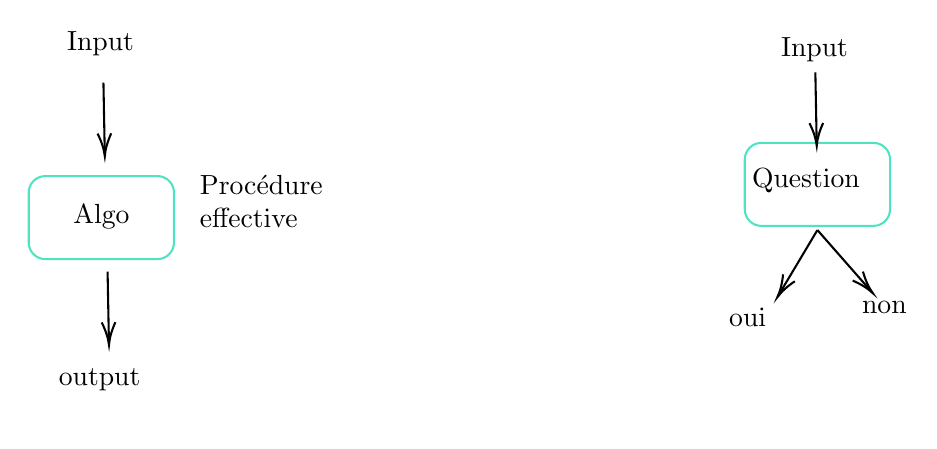
\begin{tikzpicture}[x=0.75pt,y=0.75pt,yscale=-1,xscale=1]
%uncomment if require: \path (0,300); %set diagram left start at 0, and has height of 300

%Straight Lines [id:da12189220483816354] 
\draw    (111,84) -- (111.63,117.4) ;
\draw [shift={(111.67,119.4)}, rotate = 268.92] [color={rgb, 255:red, 0; green, 0; blue, 0 }  ][line width=0.75]    (10.93,-3.29) .. controls (6.95,-1.4) and (3.31,-0.3) .. (0,0) .. controls (3.31,0.3) and (6.95,1.4) .. (10.93,3.29)   ;
%Rounded Rect [id:dp6724860737390415] 
\draw  [color={rgb, 255:red, 80; green, 227; blue, 194 }  ,draw opacity=1 ] (75,137) .. controls (75,132.58) and (78.58,129) .. (83,129) -- (137,129) .. controls (141.42,129) and (145,132.58) .. (145,137) -- (145,161) .. controls (145,165.42) and (141.42,169) .. (137,169) -- (83,169) .. controls (78.58,169) and (75,165.42) .. (75,161) -- cycle ;
%Straight Lines [id:da7505735676361531] 
\draw    (113,175) -- (113.63,208.4) ;
\draw [shift={(113.67,210.4)}, rotate = 268.92] [color={rgb, 255:red, 0; green, 0; blue, 0 }  ][line width=0.75]    (10.93,-3.29) .. controls (6.95,-1.4) and (3.31,-0.3) .. (0,0) .. controls (3.31,0.3) and (6.95,1.4) .. (10.93,3.29)   ;
%Rounded Rect [id:dp2740339183716237] 
\draw  [color={rgb, 255:red, 80; green, 227; blue, 194 }  ,draw opacity=1 ] (420,121) .. controls (420,116.58) and (423.58,113) .. (428,113) -- (482,113) .. controls (486.42,113) and (490,116.58) .. (490,121) -- (490,145) .. controls (490,149.42) and (486.42,153) .. (482,153) -- (428,153) .. controls (423.58,153) and (420,149.42) .. (420,145) -- cycle ;
%Straight Lines [id:da29169806821167166] 
\draw    (454,79) -- (454.63,112.4) ;
\draw [shift={(454.67,114.4)}, rotate = 268.92] [color={rgb, 255:red, 0; green, 0; blue, 0 }  ][line width=0.75]    (10.93,-3.29) .. controls (6.95,-1.4) and (3.31,-0.3) .. (0,0) .. controls (3.31,0.3) and (6.95,1.4) .. (10.93,3.29)   ;
%Straight Lines [id:da06188763678807363] 
\draw    (455,155) -- (436.69,185.68) ;
\draw [shift={(435.67,187.4)}, rotate = 300.82] [color={rgb, 255:red, 0; green, 0; blue, 0 }  ][line width=0.75]    (10.93,-3.29) .. controls (6.95,-1.4) and (3.31,-0.3) .. (0,0) .. controls (3.31,0.3) and (6.95,1.4) .. (10.93,3.29)   ;
%Straight Lines [id:da6168041041911708] 
\draw    (455,155) -- (480.35,183.9) ;
\draw [shift={(481.67,185.4)}, rotate = 228.74] [color={rgb, 255:red, 0; green, 0; blue, 0 }  ][line width=0.75]    (10.93,-3.29) .. controls (6.95,-1.4) and (3.31,-0.3) .. (0,0) .. controls (3.31,0.3) and (6.95,1.4) .. (10.93,3.29)   ;

% Text Node
\draw (92,58) node [anchor=north west][inner sep=0.75pt]   [align=left] {Input\\};
% Text Node
\draw (95,141) node [anchor=north west][inner sep=0.75pt]   [align=left] {Algo};
% Text Node
\draw (88,220) node [anchor=north west][inner sep=0.75pt]   [align=left] {output\\};
% Text Node
\draw (156,127) node [anchor=north west][inner sep=0.75pt]   [align=left] {Procédure\\effective};
% Text Node
\draw (436,61) node [anchor=north west][inner sep=0.75pt]   [align=left] {Input\\};
% Text Node
\draw (422,124) node [anchor=north west][inner sep=0.75pt]   [align=left] {Question};
% Text Node
\draw (411,191) node [anchor=north west][inner sep=0.75pt]   [align=left] {oui};
% Text Node
\draw (475,188) node [anchor=north west][inner sep=0.75pt]   [align=left] {non};


\end{tikzpicture}

\end{centering}

Tout l'intéret sera de savoir si on peut trouver un algorithme qui répond à une question en temps fini (qui ne boucle pas) .
Il nous faut donc formaliser toutes ces notions. 

\begin{definition}[mot]
    C'est un ensemble de symboles finis, que l'on peut concaténer pour former des chaînes de caractères.
\end{definition}

\begin{definition}
    Un alphabet $\Sigma^*$ est l'ensemble de tout les mots finis ( dont le mot vide) formé par les lettres (symboles) d'un ensemble nommé dictionnaire et noté $\Sigma$
\end{definition}

Un \textbf{Input} d'un algorithme doit être finiement représentable. Par exemple $\N$ est un input infini mais représenté par un symbole.
En fait, 
$$
x\mapsto \operatorname{enc(x)\in \Sigma^*}
$$

Etant donné un mot $w\in \Sigma^*$, décider le problème $\mathcal{P}$
revient à décider si $w\in \mathcal{L}_\mathcal{P}$ où
$$
\mathcal{L}_\mathcal{P} := \{\operatorname{x} | x \text{ est une instance positive de }\mathcal{P}\}
$$

Pour être clair, une instance positive est l'ensemble des inputs dont la question à été répondu favorablement.

\begin{exemple}
    Etant donné un mot binaire, contient- il le facteur "101" ?
    On est avec l'aplhabet $\Sigma = \{0,1\}$ et $\mathcal{L}_{101} = \{w\in \sigma^* | w \text{ contient le facteur "101"}\}$
    On peut réflechir à un algorithme pour déterminer si un mot appartient à $ \mathcal{L}_{101}$. La notion de mémoire apparait !
\end{exemple}

\begin{definition}
    On  définit un systeme formel $S$ comme la réunion d'un alphabet, synthaxe, sémantique et ect..
\end{definition}

Avec $\varphi, \pi$ dans un système $S$, où $\varphi$ est un ennoncé et $\pi$ est une tentative de preuve. On s'interresse à
$$
V_S = \{\langle \varphi, \pi \rangle | \pi \text{ est une preuve valide de } \varphi\text{ dans } S \}
$$

Pour cela, on doit s'interresser à $T_S = \{\varphi | \exists \text{ une preuve } \pi \text{ dans } S\}$
Il faut distinguer que en pratique on peut même s'il n'existe pas de preuve avec certains inputs sur d'autres input on pourrait trouver une preuve.
Il faut distingué la \textbf{vérité} et la \textbf{démontrabilité} parfois les notions sémentiques et la notion synthaxique d'une preuve ne peuvent pas toujours correspondre.


